\section{Exact endpoint and perturbation inputs}\label{app:inputs}
These stored floating-point inputs identify the calculation; their full decimal expansions are not claims of physical precision. The reconstructed endpoint centre is
\begin{equation}\label{eq:coords}
 \begin{aligned}
 T_*&=0.051955058120691594,&\quad\Dstar&=1.6925900731329657,\\
 q_*&=0.9791506418402958,&h_*&=1.3985886221312929.
 \end{aligned}
\end{equation}
The empirical uncertainty rectangle has component half-widths
\begin{equation}\label{eq:rho}
 \bm\rho=(1.225571985\times10^{-8},\ 4.011468456\times10^{-8},
 \ 1.061632250\times10^{-7},\ 1.824801669\times10^{-8}).
\end{equation}

The fixed wavevector and Fourier coefficients are
\begin{align}\label{eq:witness}
 K&=0.909013301211145,\\
 v_A&=-0.13502199918443586,\qquad
 v_P=-0.9908426008888789\,i.
\end{align}
Thus
\begin{equation}\label{eq:profile}
 a(x)=-0.270043998368872\cos Kx,\qquad
 b(x)=1.981685201777758\sin Kx.
\end{equation}

Equivalently, $\eta_+=v_A+iv_P\simeq0.8558206017$ and $\eta_-=v_A^*+iv_P^*\simeq-1.1258646001$, with sidebands at $q_*\pm K$.

\begin{table}[tbp]\centering
\caption{Stored central coefficients and allowances. Numerical radii exclude $E_{\mathrm{ep}}=3.1623619986044952\times10^{-6}$, which is added once to obtain each empirical upper endpoint. Full machine-readable records accompany the article.}\label{tab:rawresults}
\begin{tabular}{lrr}\toprule
Quantity & Central coefficient & Numerical radius\\\midrule
Gaussian & $-6.5287829634528\times10^{-5}$ & $5.8505237960874744\times10^{-8}$\\
Second linear & $-6.528782574296713\times10^{-5}$ & $1.6766293751752474\times10^{-7}$\\
$C(0.01)$ & $-2.7863363462\times10^{-5}$ & $4.0957803644\times10^{-6}$\\
$C(0.005)$ & $-5.5932063990\times10^{-5}$ & $1.1726568826\times10^{-6}$\\
$C(0.0025)$ & $-6.2948907422\times10^{-5}$ & $4.4420405631\times10^{-7}$\\
Final Richardson & $-6.528785523193218\times10^{-5}$ & $1.66327681097\times10^{-5}$\\\bottomrule
\end{tabular}
\end{table}

\begin{flushleft}
The control allowance is $2.0319595130\times10^{-7}$. The two Richardson centres are $-6.528829749948777\times10^{-5}$ and $-6.528785523193218\times10^{-5}$. Origin-shift differences at decreasing amplitudes are $2.7802392560\times10^{-9}$, $6.9433639003\times10^{-10}$, and $1.7353873522\times10^{-10}$; their allowed sums of numerical errors are $9.5198562301\times10^{-6}$, $2.6777244933\times10^{-6}$, and $9.7165279423\times10^{-7}$.
\end{flushleft}

\section{Functional consistency and endpoint derivatives}\label{app:functional}
\subsection{Amplitude and twist differentiation}
Equation~\eqref{eq:uniformF} gives $\partial_D\Omega=D/\Omega$ and therefore
\begin{equation}
 \partial_Df=2D\ln T+2\pi TD\sum_{n\ge0}
 \left[\frac{2}{\omega_n}-\sum_\lambda W_\lambda
 \operatorname{Re}\av{\Omega^{-1}}\right].
\end{equation}
At $h=q=0$, $\sum_\lambda W_\lambda=2$ and $\Omega=\sqrt{\omega_n^2+D^2}$. Dividing by $2D$ yields
\begin{equation}
 \ln T+2\pi T\sum_{n\ge0}
 \left(\frac{1}{\omega_n}-\frac{1}{\sqrt{\omega_n^2+D^2}}\right)=0,
\end{equation}
the standard transition-temperature-subtracted uniform gap equation in these units. A spurious extra factor of $T$ multiplying the logarithm would fail this check. Source plotting conventions also require care: where the source uses $\xi=v_F/|\Delta_q|$ and scales field by $|\Delta_q|$, its plotted momentum and field correspond to $q/D$ and $h/D$, rather than the $\Tc$-scaled $q,h$ used in this manuscript. The reconstructed coordinates must not be directly identified with those source-figure abscissae. The derivation also distinguishes $N_0$ from the total density of states.

For the twist, $\partial_qz=(i/2)\cos\theta$ and $\partial_q\Omega=(z/\Omega)\partial_qz$. Since $\operatorname{Re}(iX)=-\operatorname{Im}X$ and $\operatorname{Re}\partial_qz=0$, differentiating the negative determinant contribution gives Eq.~\eqref{eq:current}. This fixes the current/free-energy normalization without fitting a response prefactor to the final negative mode.

\subsection{Total versus partial endpoint derivatives}
Set $s=D'(q)=-f_{Dq}/f_{DD}$. Along the gap branch,
\begin{equation}
 g'=f_q,\qquad
 g''=f_{qq}-\frac{f_{qD}^2}{f_{DD}},\qquad
 g'''=f_{qqq}+3f_{qqD}s+3f_{qDD}s^2+f_{DDD}s^3.
\end{equation}
These are total derivatives after amplitude relaxation. Replacing them by fixed-$D$ derivatives would locate a different object. The endpoint calculation uses a four-variable root and gives an infinity-norm condition estimate of about $124.636$. Its coordinate uncertainty includes numerical refinements and solver effects rather than being identified with the central residual alone.

The central dimensionless free energy is $f_*=-0.63217093656$. The saved uniform amplitude derivative and twist derivative are near zero, but $f_{qq}\simeq0.08498845757$ is positive: it is the relaxed combination $g''$, not $f_{qq}$ by itself, that vanishes. This illustrates the importance of distinguishing a restricted variable change from the relaxed branch condition. The spatial perturbation is a further, different enlargement of the variation space.

\section{Detailed response construction}\label{app:response}
\subsection{Two representations of the local pairing response}
The primary response is the second variation of the source-compatible mean-field functional. In the background-helix gauge, write $p=\bm K\cdot\widehat{\bm k}$ and $L=4\Omega^2+p^2$, using dimensionless $v_F=1$. In the Cartesian amplitude/imaginary-pairing basis the Hermitian $2\times2$ matrix is
\begin{align}\label{eq:kernelAA}
 M_{AA}(\bm K)&=2\ln T+2\pi T\sum_{n\ge0}\left[\frac{2}{\omega_n}
 -\sum_\lambda W_\lambda\operatorname{Re}\av{\frac{4z^2}{\Omega L}}\right],\\
 M_{PP}(\bm K)&=2\ln T+2\pi T\sum_{n\ge0}\left[\frac{2}{\omega_n}
 -\sum_\lambda W_\lambda\operatorname{Re}\av{\frac{4\Omega}{L}}\right],\label{eq:kernelPP}\\
 M_{AP}(\bm K)&=-4\pi iT\sum_{n\ge0,\lambda}W_\lambda
 \av{p\operatorname{Im}\left(\frac{z}{\Omega L}\right)},
 \qquad M_{PA}=M_{AP}^*.\label{eq:kernelAP}
\end{align}
These are derived source-compatible response equations, not quotations from the source paper. The band, angular, and ultraviolet conventions are those in Section~\ref{sec:model}. The response coefficient is $\bm v^\dagger M\bm v$ for the physical harmonics in Eqs.~\eqref{eq:ab}--\eqref{eq:witness}.

The radial reduction in the underlying two-propagator calculation uses
\begin{equation}\label{eq:radial}
 \int_{-\infty}^{\infty}\frac{\dd\xi}{A_+A_-}
 =\frac{2\pi}{\Omega(4\Omega^2+p^2)},\qquad
 \int_{-\infty}^{\infty}\frac{\xi^2\dd\xi}{A_+A_-}
 =\frac{\pi}{2\Omega},\qquad
 A_\pm=(\xi\pm p/2)^2+\Omega^2.
\end{equation}
The analytic branch prescription accompanies these identities. The matrix has amplitude and imaginary-pairing vertices corresponding to $\tau_x$ and $-\tau_y$ in the Nambu convention of the constructed functional. An arbitrary positive prefactor would leave the sign unchanged, but would fail the required quantitative comparison with nonlinear free-energy differences.

The second response representation uses the spatial quasiclassical equations, expressed through two Riccati coherence sectors. Quasiclassical transport and coherence parametrizations are established tools~\cite{Eilenberger1968,Eschrig2000}; the two-sector expansion, source-domain controls, and normalized-force implementation described below specify the representation used in this calculation. Both representations share the physical model and endpoint inputs.

\subsection{Normalization and source controls before the spatial test}
At $K=0$, the matrix must reproduce the uniform Cartesian second variations,
\begin{equation}\label{eq:ward}
 M_{AA}(0)=f_{DD},\qquad M_{PP}(0)=\frac{f_D}{D}.
\end{equation}
The second identity is the phase Ward control. The measured residual is retained rather than replacing the right-hand side by zero by hand. The mixed response at small $K$ is checked against the twist--amplitude derivative in the same normalization. Additional retained controls compare the raw source response, the signed force, current and free-energy derivatives, zero-field limits, and Hermiticity.

\subsection{Periodic Riccati expansion with complete Fourier support}
For one helicity, trajectory, and positive Matsubara frequency, the uniform coherence amplitude is
\begin{equation}
 a_0=\frac{D}{z+\Omega}.
\end{equation}
At signed physical perturbation amplitude $\beta$, write the two coherence sectors as
\begin{equation}\label{eq:riccati}
 A_\beta=a_0+\beta U_\beta,\qquad
 B_\beta=a_0+\beta V_\beta.
\end{equation}
Both sectors use the same causal $z$. The second sector reverses transport and conjugates the prescribed pairing profile; it does not replace $z$ by $z^*$. This distinction is necessary when the field and phase twist produce a complex Matsubara shift.

Expanding $U_\beta=\sum_{k\ge0}\beta^k U_k$, the Fourier inverse has denominator $2\Omega+imp$. With $\mathcal L_m=2\Omega+imp$, the recurrence can be written
\begin{align}\label{eq:recurrence}
 \mathcal L U_0&=\eta-a_0^2\eta^*,\\
 \mathcal L U_k&=-2a_0\eta^*U_{k-1}
 -D\!\sum_{i+j=k-1}U_iU_j
 -\eta^*\!\sum_{i+j=k-2}U_iU_j\quad(k\ge1).
\end{align}
The $V$ sector uses the conjugate profile and the opposite transport denominator. Empty sums vanish. At each order, every convolution mode generated by the recurrence is retained; for a first-harmonic forcing the support grows to $|m|\le k+1$. Products are evaluated by full finite Fourier convolution rather than by a spatial collocation grid that could fold modes back into the retained range.

The spatial mean of the retained polynomial is exactly its zero Fourier coefficient. ``Exact'' here describes the finite Fourier averaging identity, not an exact arithmetic evaluation or a claim that the infinite response is a finite polynomial. Omitted perturbative orders and their Fourier content remain in the residual and analytic remainder estimates.

\subsection{Normalized anomalous force and energy-path integration}
The normalized force has two denominator factors. Defining
\begin{equation}
 Q=1+a_0^2,\qquad h_\beta=\beta a_0(U_\beta+V_\beta)+\beta^2U_\beta V_\beta,
\end{equation}
the divided anomalous response is
\begin{equation}\label{eq:dividedforce}
 \mathcal A_\beta=
 \frac{2\left(U_\beta-a_0^2V_\beta-\beta a_0U_\beta V_\beta\right)}
 {Q\left(Q+h_\beta\right)}.
\end{equation}
The finite denominator $Q+h_\beta$ and the background factor $Q$ both enter the force estimates. Bounding only one would not control the normalized physical response. The scalar force contribution is the real spatial zero mode of $\eta^*\mathcal A_\beta$, denoted $\mathcal G_\beta$.

Instead of subtracting two independently accumulated large thermodynamic potentials, the nonlinear coefficient is assembled as a correction to the matched linear coefficient:
\begin{equation}\label{eq:path}
 C(\epsilon)=c_0-\pi T\sum_{n\ge0,\lambda}W_\lambda
 \av{\sum_{\sigma=\pm1}\int_0^1
 t\left[\mathcal G_{\sigma t\epsilon}-\mathcal G_0\right]\dd t}.
\end{equation}
The log and $1/\omega_n$ counterterms cancel in this correction; they are already present in the second linear baseline. The source-dependent $\pi T$ prefactor remains explicit. The anchor's numerical allowance is included once in the complete quotient error.

Path integration is checked against closed polynomial moments. A term proportional to $\beta^k$ contributes the moment $\int_0^1 t^{k+1}\dd t=1/(k+2)$. The paired signs remove odd orders before error magnitudes are formed. Gaussian path-node refinement is retained as a numerical control, and the path-polynomial discrepancy is propagated rather than assumed to vanish.

The norm used in analytic majorants is the Fourier $\ell^1$ norm of the forcing profile. It bounds convolution and remainder growth; it is not an additional denominator in Eq.~\eqref{eq:paired}. For the normalized two-component witness, the spatial mean of $|\eta|^2$ is two. Dividing the final energy quotient by that norm would change the normalization and destroy the match to $\bm v^\dagger M\bm v$.

\subsection{Low-frequency coverage, source uncertainty, and connected branches}
Low positive Matsubara frequencies are the numerically delicate part of the calculation. Frequencies $n<32$ use explicit source-coefficient radii, complete omitted-profile residuals, the full normalization identity, and inverse estimates that cover both the retained finite-mode block and the infinite high-mode remainder. Sixteen signed-$\beta$ cells cover $[-0.01,0.01]$; the calculated common profile remainder cap is $0.001$, with a high-mode split index of 12.

The bounds preserve a common connected uniqueness neighbourhood for the two coherence sectors and the signed amplitudes. This guards against accepting a different algebraic branch at one amplitude. Continuous angular-domain estimates cover the stated endpoint rectangle and signed-$\beta$ interval. The two angular-origin calculations share these domain estimates and the same linear baseline; this dependence is included when interpreting their comparison.

The source uncertainty is a rectangle in all four coordinates in Eq.~\eqref{eq:coords}. Its effects are propagated through the uniform background, both Riccati sectors, the normalized force, and the temperature prefactor. Evaluating only the centre, or only a few corners, would not establish the documented domain coverage. A coordinate stored exactly as a binary64 number is still the centre of a physically uncertain reconstructed state.

The endpoint-error allocation uses $\Eep$ once. The linear endpoint-variation estimate occupies $9.9246651098\times10^{-7}$; the remaining nonlinear source-correction allowance is $2.1698954876\times10^{-6}$. These add to $\Eep$. The measured nonlinear source radii are smaller than the available nonlinear allowance. They are not treated as independent random variables to be combined in quadrature with the endpoint allowance.

\subsection{High frequencies and the complete omitted Matsubara tail}
For $n\ge32$, a source-uniform complex-$\beta$ disk of radius $r=0.1$ supports analytic remainder estimates in addition to the explicitly computed finite-amplitude correction. The omitted-frequency estimate includes every higher even perturbative order after sign pairing. The tail is not set to zero at the largest computed frequency.

For a source-uniform force majorant of the form $|\mathcal G_\beta-\mathcal G_0|\le C_f/\omega^3$ on the disk, the retained paired envelope has the form
\begin{equation}\label{eq:tail}
 B_{\mathrm{tail}}\le 2\pi T_{\max} C_f
 \frac{(\epsilon/r)^2}{1-(\epsilon/r)^2}
 \left[\frac{1}{w^3}+\frac{1}{4\pi T_{\min}w^2}\right],
 \qquad w=(2N_\omega+1)\pi T_{\min},
\end{equation}
with the calculated arithmetic allowance added. The geometric factor retains all omitted even orders. $C_f$ is obtained from the source-uniform two-sector, two-pole contraction estimates, rather than fitted to a decreasing sequence of observed tail values.

At $N_\omega=512$, the saved infinite-frequency quotient-tail envelopes are approximately $1.5156907408\times10^{-6}$, $3.7607439433\times10^{-7}$, and $9.3842953931\times10^{-8}$ at $\epsilon=0.01,0.005,0.0025$. Their amplitude dependence is consistent with the correction's leading even order. They are components of the complete error budget, not the complete uncertainty by themselves.

\subsection{Five refinement axes and all mixed pairs}
A configuration is calculated as
\begin{equation}\label{eq:config}
 (J,N_\omega,N_\theta,P,N_t).
\end{equation}
The axes and their three levels are listed in Table~\ref{tab:levels}. $J$ is the retained profile expansion degree; $2P$ is the retained force expansion degree; $N_t$ controls the path rule. The angular rules use one common origin to preserve their nested hierarchy. They do not rotate the physical $q$, $\bm h$, or $\bm K$.

\begin{table}[tbp]\centering
\caption{\textbf{Numerical refinement levels.} The finest configuration is $(16,512,64,8,8)$. The schedule contains the fine centre, two lower levels along each axis, and two levels for each of ten mixed pairs, giving $1+10+20=31$ configurations. Three perturbation amplitudes give 93 rows.}\label{tab:levels}
\begin{tabular}{llrrr}\toprule
Axis & Meaning & Coarse & Medium & Fine\\\midrule
$J$ & Profile perturbation degree &8&12&16\\
$N_\omega$ & Explicit positive Matsubara frequencies &128&256&512\\
$N_\theta$ & Angular nodes &16&32&64\\
$P$ & Half the force perturbation degree &4&6&8\\
$N_t$ & Path quadrature nodes &2&4&8\\\bottomrule
\end{tabular}
\end{table}

For an axis, let $d_1$ be the medium-minus-coarse change and $d_2$ the fine-minus-medium change. The predefined rule requires $|d_2|\le0.75|d_1|+b_{\mathrm{noise}}$, with a same-sign condition unless the change is noise sized. The calculated axis allowance is constructed from the final change and the row error radii, including the form $4(|d_2|+b_1+b_2)+b_2$. Convergence ratios alone are insufficient when cancellation drives a difference close to the primitive noise floor.

Mixed contrasts detect interactions between refinements. They compare jointly changed settings with their individually changed counterparts at two levels for each axis pair. All ten pairs are tested and their allowances included. This avoids assigning the entire error to separate one-dimensional differences when, for example, profile and angular refinements interact.

The complete quotient allowance includes the second linear anchor, spatial/profile remainder, primitive arithmetic and normalized-force defects, path integration, the infinite-frequency tail, the five axis allowances, and the ten mixed allowances. It is added as an absolute radius, not interpreted as a statistical variance. The amplitude hierarchy is separately checked with its predefined contraction factor of $0.5$ plus propagated noise. The Richardson check has its own complete allowance.

\subsection{Numerical criteria and angular-origin comparison}
The local quadratic test requires both source-inclusive upper bounds to be negative, the primary and independent total radii to be at most one quarter of the respective coefficient magnitudes, and representation agreement within $E_{\mathrm P}+\EI$. The source controls must fit inside the endpoint-error allocation. The nonlinear sign test additionally requires $C_1$ and $C_2$ to remain negative beyond their complete numerical and endpoint allowances. Source and branch controls, the complete schedule, refinement and amplitude rules, tail coverage, and origin agreement are required as applicable. Unresolved numerical checks are inconclusive; they are not physical evidence for either sign.

The fresh confirmation uses
\begin{equation}\label{eq:origin}
 \theta_j=\frac{2\pi j}{N_\theta}+\phi_0,\qquad
 \phi_0=\frac{\pi\sqrt5}{256}.
\end{equation}
Every angle-dependent nonlinear response in the 93-row schedule was recomputed on this origin. Its comparison with the baseline-origin calculation shares the same physical state, linear coefficient, and continuous-domain estimates. The comparison therefore probes discretization sensitivity of the fixed direction; it is not statistical replication.

\subsection{Arithmetic and computational cost}
The calculations use binary64 real and complex128 arithmetic. Primitive error estimates include an empirical floor of $10^{-12}$; recurrence and normalization residuals are required to be at most $10^{-10}$. These tolerances enter the error estimates and are not a replacement for controlling frequency tails or endpoint-coordinate uncertainty. Vectorized coefficient contractions accelerate the recurrence and majorant calculations without changing the model or the retained Fourier support.

The complete shifted-origin calculation requires $12751.5790$ seconds of calculation CPU time and $14348.2845$ seconds elapsed, approximately 3.54 CPU hours and 3.99 elapsed hours. These costs refer to the 606208 two-sector expansions and associated numerical processing. The schedule comprises 606208 two-sector expansion nodes: 1184 at each of 512 explicit positive Matsubara frequencies. The stored angular origin is $0.02744068254312784$ radians.


\section{Detailed error accounting and acceptance arithmetic}\label{app:errors}
\subsection{Additive error decomposition}
For each amplitude, let $E_{\mathrm{fine}}$ denote the finest row's complete coefficient radius, including the second linear baseline uncertainty and explicit nonlinear components. The final complete allowance is
\begin{equation}\label{eq:EIassembled}
 E_C=E_{\mathrm{fine}}+\sum_{a=1}^5E_a
 +\sum_{1\le a<b\le5}E_{ab}.
\end{equation}
The original endpoint/source allowance $\Eep$ is then added once for the sign test. The row-specific nonlinear source radius is checked against its allocated source budget. Adding it again on top of the full $\Eep$ would double count that coverage.

At the finest row, the explicit numerical correction radius is the sum of tail, primitive, normalized-force residual, path-polynomial, and spatial terms. The aggregate quotient radius must also account for the second linear baseline and the observed refinement hierarchy. Table~\ref{tab:errorbreakdown} shows the resulting decomposition. A zero calculated spatial term applies to the retained finite-polynomial accounting; omitted modes/orders are covered by the residual and analytic estimates, not asserted absent from the physical response.

\begin{table}[tbp]\centering
\caption{Nonlinear numerical allowance decomposition. Endpoint allowance $E_{\mathrm{ep}}=3.1623619986\times10^{-6}$ is added separately and once for the sign test. Values use the normalized quotient units.}\label{tab:errorbreakdown}
\begin{tabular}{rrrrrr}\toprule
$\epsilon$ & Fine row & Five axes & Ten mixed & Total $E_C$ \\\midrule
0.0100 & $1.683720\times10^{-6}$ & $2.386198\times10^{-6}$ & $2.586194\times10^{-8}$ & $4.095780\times10^{-6}$ \\
0.0050 & $5.441040\times10^{-7}$ & $6.026909\times10^{-7}$ & $2.586194\times10^{-8}$ & $1.172657\times10^{-6}$ \\
0.0025 & $2.618726\times10^{-7}$ & $1.564696\times10^{-7}$ & $2.586194\times10^{-8}$ & $4.442041\times10^{-7}$ \\
\bottomrule\end{tabular}\end{table}


The mixed checks use saved contrasts $m_1,m_2$ and corresponding row-noise allowances $b_1,b_2$. The convergence heatmap shows the maximum of
\begin{equation}
 \frac{|m_2|}{0.75|m_1|+b_1+b_2},\qquad
 \frac{|m_2|}{0.25\sum_{\ell=1}^5E_\ell+b_2}.
\end{equation}
A value below one satisfies both magnitude conditions represented in the panel. The axis and amplitude hierarchies also retain their respective sign/noise rules; colour alone is not a substitute for the complete numerical checks.

\subsection{Source and amplitude uncertainty are distinct}
The endpoint coordinate uncertainty affects both the background linear coefficient and the nonlinear correction. Their documented source budgets are assigned so that the total stays within the original $\Eep$. Refinement errors instead measure resolution sensitivity under the fixed source domain. The two should not be combined as uncorrelated Gaussian variables.

Similarly, the difference between $C(0.005)$ and $C(0.0025)$ is primarily a finite-amplitude correction, not a sampling uncertainty. The extrapolation removes its leading even order under an analytic expansion. The complete Richardson allowance remains large enough that the sign conclusion does not depend on claiming its central-value precision as certified precision.

\subsection{Numerical consistency criteria}
The retained numerical consistency criteria are: source controls; complete axis and mixed hierarchy; complete nonlinear $C_1$ negativity; complete nonlinear $C_2$ negativity; complete Richardson negativity; complete schedule; amplitude hierarchy; normalization-control adequacy; linear-response negativity; cross-representation agreement; quarter-error rule; shifted-origin agreement; and source-budget adequacy. All of these criteria are required together for the stated conclusion. 

The formal stability implication and its numerical premise should remain separate. Conditional on an actual $c<0$ and the usual differentiability of the functional, Eq.~\eqref{eq:descent} excludes a local minimum. The present calculation supplies empirical numerical evidence for that premise in the stated model; it does not prove that all primitive errors have been enclosed for every real input by directed rounding.

\section{Reproduction recipe and complete configuration table}\label{app:repro}
The numerical calculation can be reconstructed from the physical and numerical definitions in this article. A reproduction must use the same normalization throughout; resolving a negative sign with a mismatched overall factor would not reproduce the stated coefficients.

\begin{enumerate}
\item Fix $\widetilde\alpha=1/4$, the causal positive-frequency branch, and the dimensionless units in Eq.~\eqref{eq:units}. Evaluate the uniform functional with its transition-temperature subtraction and the infinite-frequency remainder.
\item Solve the four endpoint equations in Eq.~\eqref{eq:endpoint}, using total derivatives along the amplitude-relaxed branch. Check the two coexistence minima and intermediate stationary point, positive amplitude curvature, and positive relaxed quartic. Propagate the coordinate rectangle in Eq.~\eqref{eq:rho}.
\item Fix $K,v_A,v_P$ in Eq.~\eqref{eq:witness}. Evaluate Eqs.~\eqref{eq:kernelAA}--\eqref{eq:kernelAP} and the zero-wavevector/current normalization checks. Independently evaluate the linearized Riccati response, including its full numerical error estimate.
\item For each angular rule and positive Matsubara frequency, expand both causal Riccati sectors using Eq.~\eqref{eq:recurrence}. Keep every generated Fourier convolution mode. Evaluate the normalized force in Eq.~\eqref{eq:dividedforce}, controlling both denominator factors and the omitted profile remainder.
\item Integrate the paired nonlinear correction in Eq.~\eqref{eq:path}, with the two signs and the three amplitudes. Check polynomial path moments, the source rectangle, signed-amplitude branch continuity, low-frequency residual estimates, and the complex-amplitude disk. Include the complete omitted-frequency envelope in Eq.~\eqref{eq:tail}.
\item Evaluate the 31 configurations in Table~\ref{tab:configurations}; construct single-axis changes, all ten mixed contrasts, amplitude contraction and Richardson values. Add the numerical allowances as in Eq.~\eqref{eq:EIassembled}, and add the endpoint allowance once. Compare the primary and second linear coefficients and test the strict negative upper endpoints.
\item Repeat the nonlinear angular calculation with the common shifted origin in Eq.~\eqref{eq:origin}. Compare the resulting coefficients against the sum of complete numerical allowances. This final step tests angular sensitivity while sharing the fixed state and linear baseline.
\end{enumerate}

The equations specify the functional, perturbation, expansion, force, integration path, numerical hierarchy, error composition and sign criterion. They do not convert the empirical primitive estimates into validated interval arithmetic: that limitation remains part of the reproducible result. A rigorously certified reproduction would additionally require outward-rounded primitive and accumulation bounds over the entire parameter domain.



Table~\ref{tab:configurations} reports every configuration and the three corresponding central quotients. All physical inputs are given in Eqs.~\eqref{eq:coords}, \eqref{eq:rho}, and \eqref{eq:witness}; the numerical levels are in Table~\ref{tab:levels}. Central-value digits allow numerical comparison; the appropriate uncertainty remains the complete numerical allowance plus endpoint allowance in Table~\ref{tab:nonlinear}.
\small
\begin{longtable}{rrrrrrrr}
\caption{Shifted-origin configurations and central quotients in units of $10^{-5}$. Settings follow Eq.~\eqref{eq:config}; the finest configuration is $(16,512,64,8,8)$.}\label{tab:configurations}\\
\toprule $J$ & $N_\omega$ & $N_\theta$ & $P$ & $N_t$ & $C(.01)$ & $C(.005)$ & $C(.0025)$\\\midrule\endfirsthead
\toprule $J$ & $N_\omega$ & $N_\theta$ & $P$ & $N_t$ & $C(.01)$ & $C(.005)$ & $C(.0025)$\\\midrule\endhead
\bottomrule\endfoot
8 & 128 & 64 & 8 & 8 & -2.79025510 & -5.59418609 & -6.29513566\\
8 & 512 & 16 & 8 & 8 & -2.16735454 & -5.43841537 & -6.25619014\\
8 & 512 & 64 & 4 & 8 & -2.78633635 & -5.59320640 & -6.29489074\\
8 & 512 & 64 & 8 & 2 & -2.78635207 & -5.59320738 & -6.29489080\\
8 & 512 & 64 & 8 & 8 & -2.78633635 & -5.59320640 & -6.29489074\\
12 & 256 & 64 & 8 & 8 & -2.78712183 & -5.59340277 & -6.29493983\\
12 & 512 & 32 & 8 & 8 & -2.72765934 & -5.57852796 & -6.29122056\\
12 & 512 & 64 & 6 & 8 & -2.78633635 & -5.59320640 & -6.29489074\\
12 & 512 & 64 & 8 & 4 & -2.78633635 & -5.59320640 & -6.29489074\\
12 & 512 & 64 & 8 & 8 & -2.78633635 & -5.59320640 & -6.29489074\\
16 & 128 & 16 & 8 & 8 & -2.17127330 & -5.43939506 & -6.25643506\\
16 & 128 & 64 & 4 & 8 & -2.79025510 & -5.59418609 & -6.29513566\\
16 & 128 & 64 & 8 & 2 & -2.79027083 & -5.59418707 & -6.29513573\\
16 & 128 & 64 & 8 & 8 & -2.79025510 & -5.59418609 & -6.29513566\\
16 & 256 & 32 & 8 & 8 & -2.72844482 & -5.57872433 & -6.29126965\\
16 & 256 & 64 & 6 & 8 & -2.78712183 & -5.59340277 & -6.29493983\\
16 & 256 & 64 & 8 & 4 & -2.78712183 & -5.59340277 & -6.29493983\\
16 & 256 & 64 & 8 & 8 & -2.78712183 & -5.59340277 & -6.29493983\\
16 & 512 & 16 & 4 & 8 & -2.16735454 & -5.43841537 & -6.25619014\\
16 & 512 & 16 & 8 & 2 & -2.16735001 & -5.43841509 & -6.25619012\\
16 & 512 & 16 & 8 & 8 & -2.16735454 & -5.43841537 & -6.25619014\\
16 & 512 & 32 & 6 & 8 & -2.72765934 & -5.57852796 & -6.29122056\\
16 & 512 & 32 & 8 & 4 & -2.72765934 & -5.57852796 & -6.29122056\\
16 & 512 & 32 & 8 & 8 & -2.72765934 & -5.57852796 & -6.29122056\\
16 & 512 & 64 & 4 & 2 & -2.78635207 & -5.59320738 & -6.29489080\\
16 & 512 & 64 & 4 & 8 & -2.78633635 & -5.59320640 & -6.29489074\\
16 & 512 & 64 & 6 & 4 & -2.78633635 & -5.59320640 & -6.29489074\\
16 & 512 & 64 & 6 & 8 & -2.78633635 & -5.59320640 & -6.29489074\\
16 & 512 & 64 & 8 & 2 & -2.78635207 & -5.59320738 & -6.29489080\\
16 & 512 & 64 & 8 & 4 & -2.78633635 & -5.59320640 & -6.29489074\\
16 & 512 & 64 & 8 & 8 & -2.78633635 & -5.59320640 & -6.29489074\\
\end{longtable}
\normalsize


\FloatBarrier
\section{Diagnostic figures}
\begin{figure}[tbp]\centering
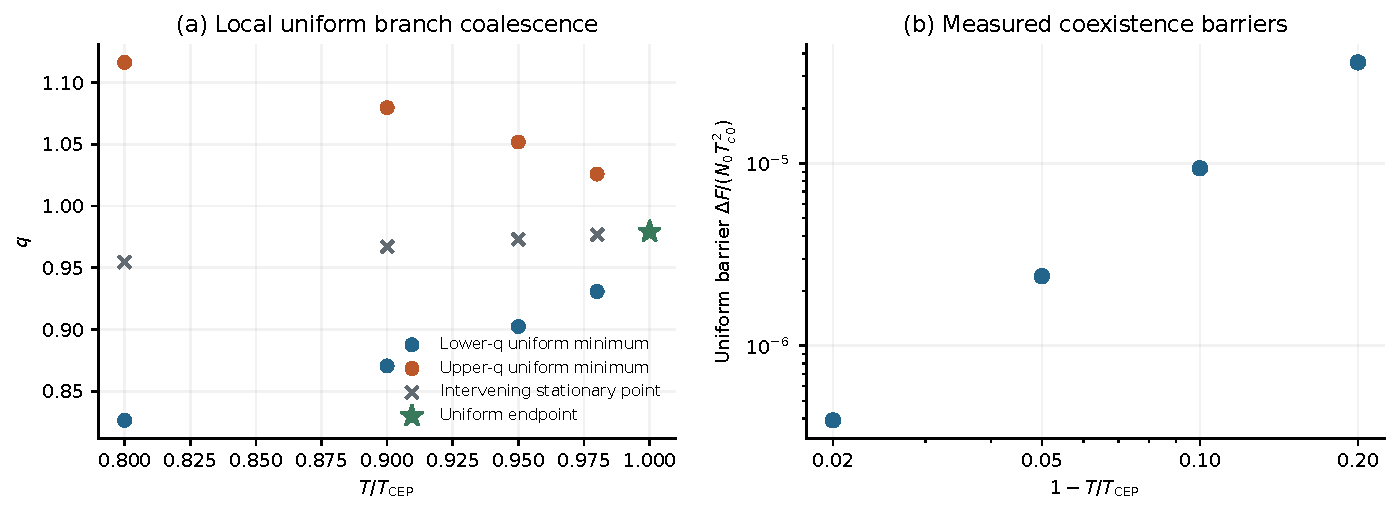
\includegraphics[width=\textwidth]{figures/fig01_endpoint_topology.pdf}
\caption{Restricted uniform endpoint topology. Samples at four temperatures between $0.80T_*$ and $0.98T_*$ show the two coexistence minima and intervening stationary point; the right panel gives uniform barriers. The field varies along coexistence, and connecting samples does not establish a fixed-field scan or fitted critical law.}\label{fig:endpoint}
\end{figure}
\begin{figure}[tbp]\centering
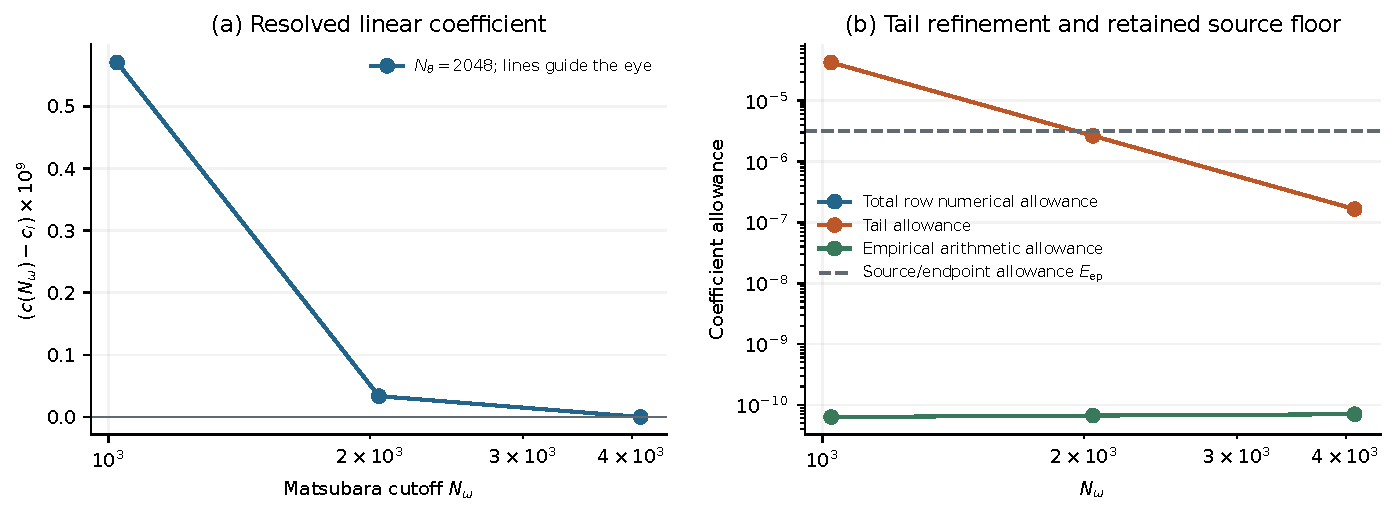
\includegraphics[width=\textwidth]{figures/fig02_linear_qualification.pdf}
\caption{Second quadratic-response representation under frequency refinement at $N_\theta=2048$. Coefficients are measured relative to the finest row; the right panel separates row numerical, tail, and primitive-arithmetic radii from the endpoint allowance. The final allowance also includes single- and mixed-refinement contributions.}\label{fig:linear}
\end{figure}
\begin{figure}[tbp]\centering
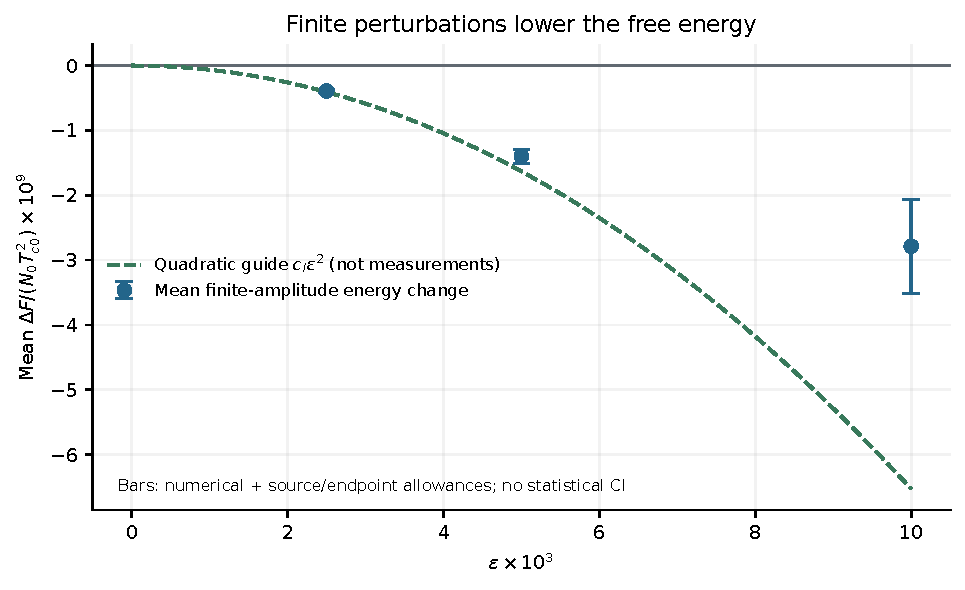
\includegraphics[width=\textwidth]{figures/fig04_energy_descent.pdf}
\caption{Paired mean energy change $\overline{\delta f}=\epsilon^2C$ in units of $N_0\Tc^2$, reconstructed from the computed quotients with radius $\epsilon^2(E_C+E_{\mathrm{ep}})$. The dashed $\cI\epsilon^2$ curve is a quadratic guide. A negative paired mean ensures a descending signed member without assigning equal lowering to both signs.}\label{fig:energy}
\end{figure}
\begin{figure}[tbp]\centering
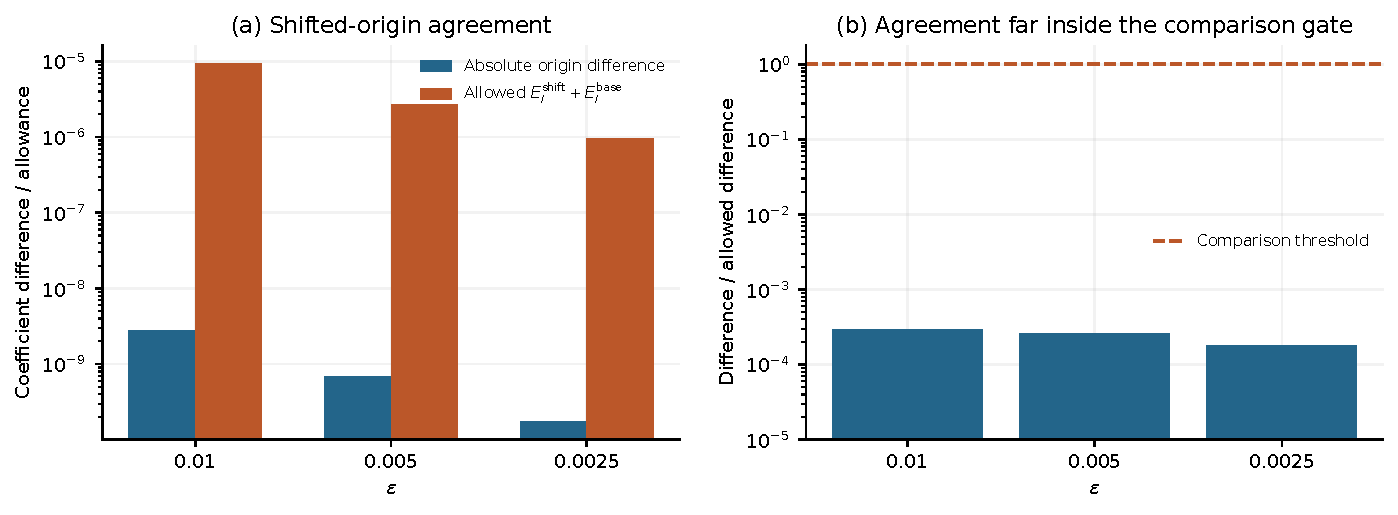
\includegraphics[width=\textwidth]{figures/fig05_origin_agreement.pdf}
\caption{Angular-origin sensitivity. Absolute quotient differences after shifting the origin by $\pi\sqrt5/256$ are smaller than the sum of complete numerical allowances. The comparison shares the physical direction, linear baseline, and domain estimates; common endpoint uncertainty is excluded from the difference allowance.}\label{fig:origin}
\end{figure}
\begin{figure}[tbp]\centering
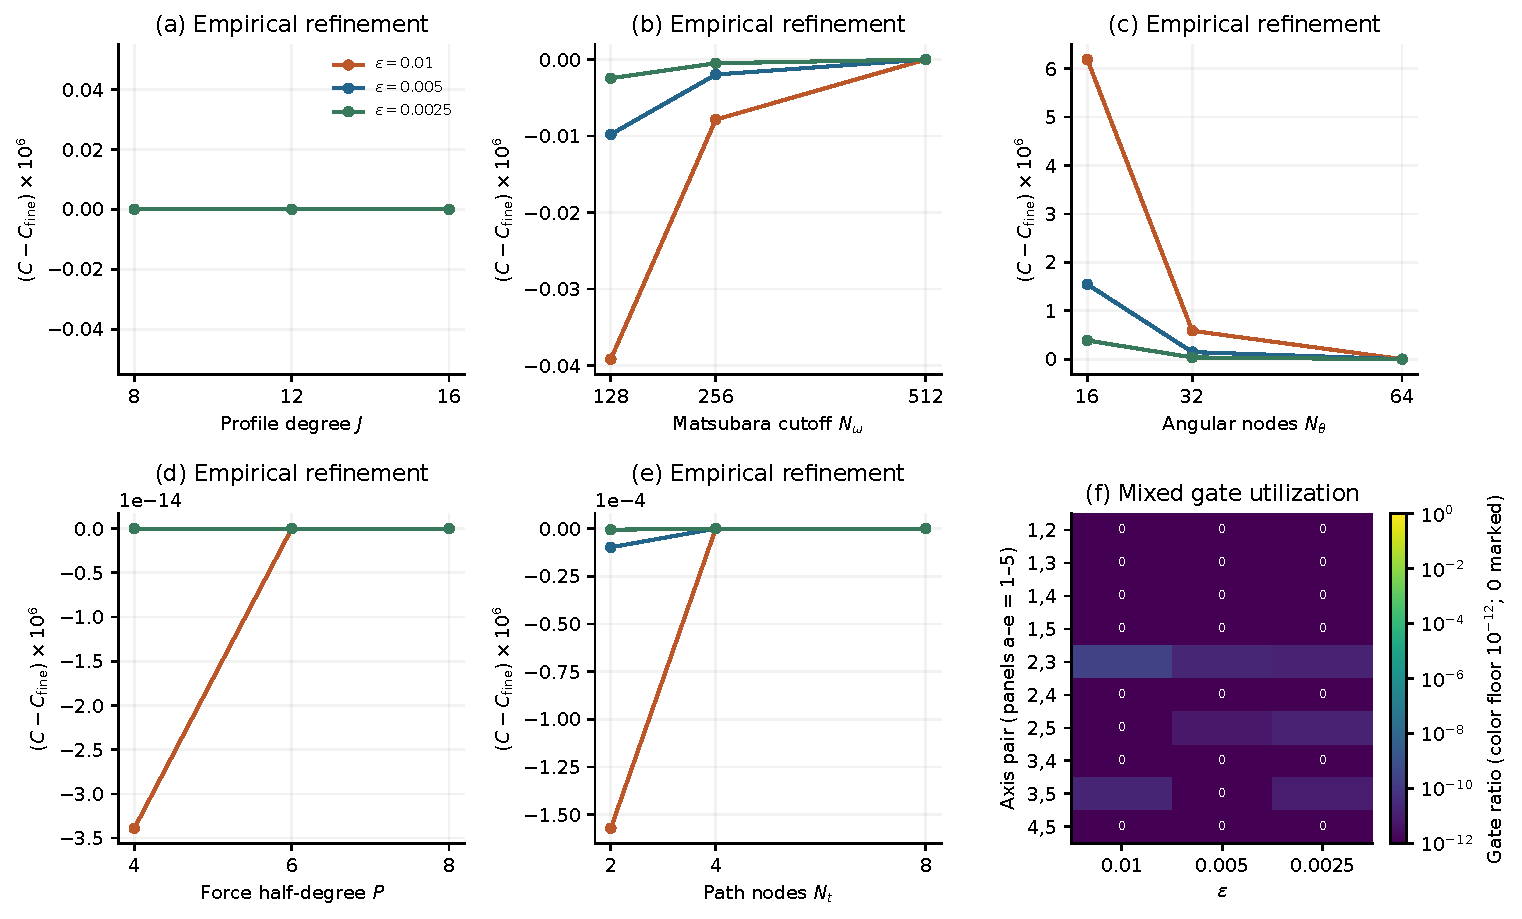
\includegraphics[width=\textwidth]{figures/fig06_axis_mixed_convergence.pdf}
\caption{Single- and mixed-refinement diagnostics. Single-axis changes relative to the finest row are shown in units of $10^{-6}$, with axis definitions in Table~\ref{tab:levels}. The final panel gives the larger utilization of the two inequalities in Appendix~\ref{app:errors}; values below $10^{-12}$ share the lowest colour, and computed exact zeros are marked.}\label{fig:axes}
\end{figure}
\FloatBarrier

